\chapter{Pruebas y Resultados}
\spacing{1.5}
\section{Pruebas}
Para las pruebas realizadas se utilizó una computadora con un procesador AMD Phenom II 720 con tres núcleos a 2.80Ghz cada núcleo, 10 GB de memoria RAM y una tarjeta gráfica NVIDIA GeForce GTX 650 Ti tiene una arquitectura Kepler con 768 núcleos CUDA, memoria de 2 GB y un ancho de banda para 86.4 GB/s. En cuanto al software las pruebas de hicieron bajo un sistema operativo xubuntu 14.04, utilizando openCV y CUDA 6.5.\\
Teniendo en cuenta el hardware y la forma en que se diseñaron los kernels se deben realizar ciertas optimizaciones. Para esta implementación como no se usa memoria compartida le daremos preferencia a la memoria cache L1 usando, la función \textbf{cudaFuncSetCacheConfig()} recibe 2 parámetros el primero será el nombre de la función del dispositivo (kernel) y el segundo es la configuración que se le dará a la memoria, en este caso \textit{cudaFuncCachePreferL1}. Además, se debe tomar en cuenta la ocupación de los SM definida por la relación entre los \textit{warps} activos y la cantidad de \textit{warps} por SM. NVIDIA desarrollo una herramienta llamada CUDA Occupancy Calculator\cite{calc}, la cual auxilia al desarrollador a encontrar la máxima ocupación para el lanzamiento de un kernel. Necesitará como datos de entrada el número de hilos por bloque, la cantidad de memoria compartida usada y el número de registros por hilo.\\\\\\
Otra herramienta que resulta muy útil para identificar problemas de rendimiento es el perfilador visual de NVIDIA\cite{profile}, gracias a este se pudo analizar la ocupación teórica calculada contra la real para cada ejecución de los diferentes kernel lanzados con diferentes imágenes de entrada, como se puede ver en la tabla 5-1.\\
\begin{table}[H]
\centering
\begin{tabular}{|l|c|c|c|}
\hline
\multicolumn{4}{|c|}{Ocupación de los SM} \\
\cline{1-4}
Kernel & Teórica &  Máxima Real &  Mínima Real\\
\hline \hline
 Convolución                    & 100\%   &  99\%   &   13\%                     \\ \cline{1-4}
 Localización de min-max        & 100\%   &  93\%   &   12\% \\ \cline{1-4}
 Remover puntos malos           & 100\%   &  93\%   &   28\%                \\ \cline{1-4}
 Asignar magnitud y orientación & 100\%   &  84\%   &   32\%            \\ \cline{1-4}
 Puntos característicos         & 56\%    &  55\%   &   1.7\%           \\ \cline{1-4}
\end{tabular}
\caption{Ocupación teórica vs ocupación real}
\label{tabla:final}
\end{table}
Una vez dicho como se encontró la mejor condición de lanzamiento y distribución de la memoria para cada kernel, se puede describir como se realizaron las pruebas en general. Las pruebas se realizaron tomando un grupo de imágenes de diferentes resoluciones como entrada de la implementación propuesta, para medir el tiempo que le tomaba procesar la imagen y compararlo con otras implementaciones del algoritmo SIFT, ya existentes. La razón de porque imágenes de distintas resoluciones es por la manera tan diversa de obtener imágenes en el robot Justina.\\\\\\\\\\\\
\section{Resultados}
Hay dos imágenes que fueron las que ayudaron a realizar paso a paso el desarrollo de la implementación propuesta, la primera imagen es un castor, y la segunda imagen de un gato (figura 5-1). La razón por la cual se tomaron estas dos imágenes fue porque la imagen del castor es una imagen pequeña con pocos puntos característicos, y la del gato siendo de una resolución mayor y con una gran cantidad de puntos característicos. Siendo estas dos imágenes los extremos en cuanto a los datos de entrada.\\

\begin{figure}[H]
    \centering
    \begin{subfigure}[b]{0.4\textwidth}
        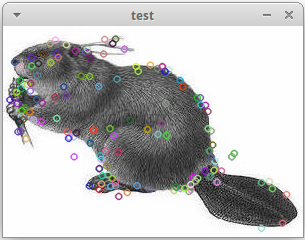
\includegraphics[width=\textwidth]{img/castor.png}
        \caption{Castor}
    \end{subfigure}
    ~ %add desired spacing between images, e. g. ~, \quad, \qquad, \hfill etc. 
      \begin{subfigure}[b]{0.4\textwidth}
        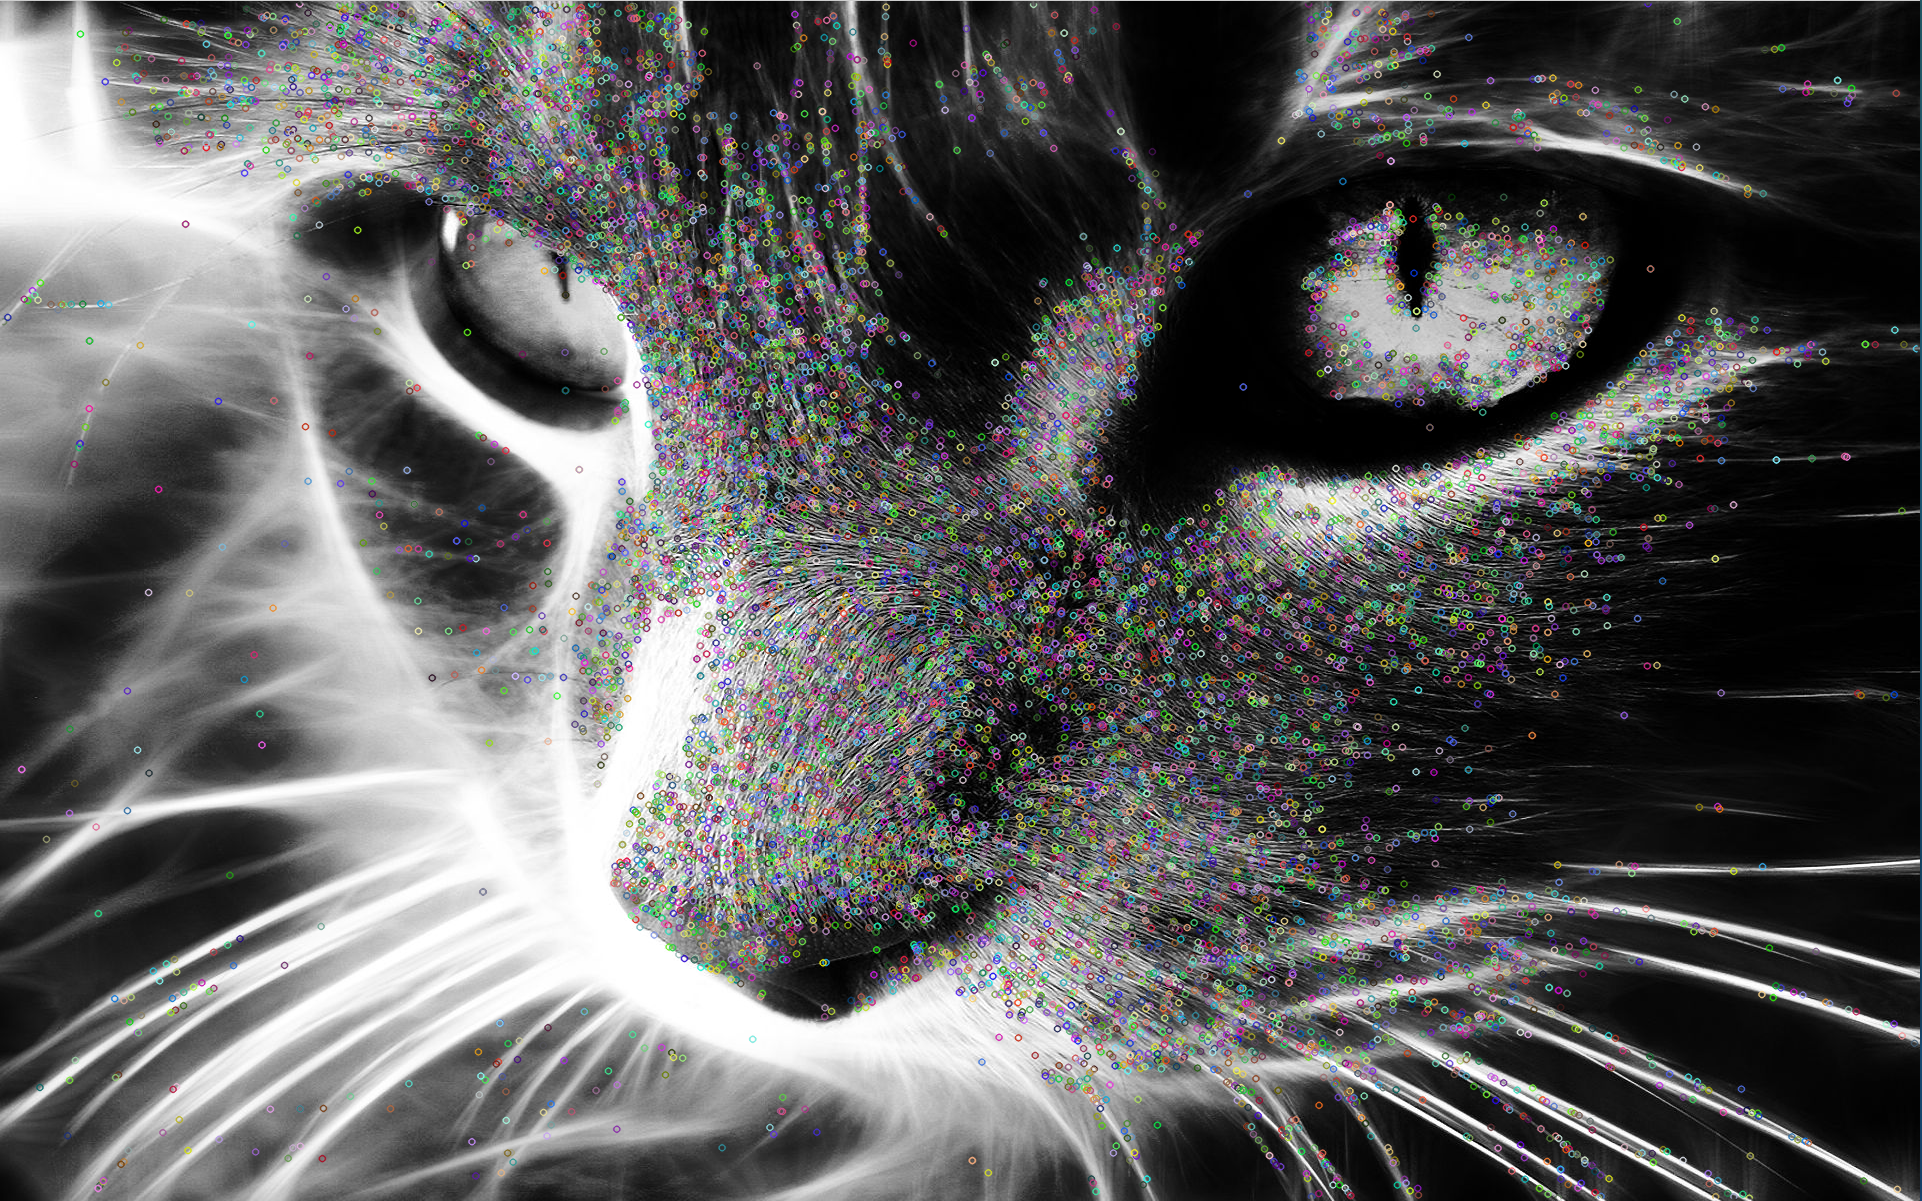
\includegraphics[width=\textwidth]{img/gato.png}
        \caption{Gato}
    \end{subfigure}
    \caption{Puntos característicos encontrados }
\end{figure}



La primer prueba que se hizo con el castor y el gato, consistió en medir el tiempo que tardaban en ejecutarse ciertas secciones del código de una implementación abierta de SIFT llamada Open SIFT \cite{OpenSIFT}, la cual se usa para la detección de objetos en el robot Justina, y en la implementación de SIFT con CUDA realizada para obtener los puntos característicos. Se puede observar en las tablas 5-2 y 5-3 los resultados de estas pruebas.\\
\begin{table}[H]
\centering
\begin{tabular}{|l|c|c|}
\hline
\multicolumn{3}{|c|}{Castor} \\
\cline{1-3}
Partes de SIFT & CUDA SIFT & Open SIFT\\
\hline \hline
 Espacio escala DoG      & 17.25 ms   &  29.32 ms                        \\ \cline{1-3}
 Detección y filtrado de PC & 2.62 ms   &  50.09 ms    \\ \cline{1-3}
 Orientación de PC       & 8.80 ms   &  12.35 ms                        \\ \cline{1-3}
\end{tabular}
\caption{La resolución de la imagen es de 300x211 px y se encontraron 120 puntos característicos}
\label{tabla:final}
\end{table}
\begin{table}[H]
\centering
\begin{tabular}{|l|c|c|}
\hline
\multicolumn{3}{|c|}{Gato} \\
\cline{1-3}
Partes de SIFT & CUDA SIFT & Open SIFT\\
\hline \hline
 Espacio escala DoG         & 473.33 ms  &  957.19 ms                       \\ \cline{1-3}
 Detección y filtrado de PC & 65.29 ms   &  2210.82 ms                       \\ \cline{1-3}
 Orientación de PC          & 125.2 ms   &  1014.89 ms                      \\ \cline{1-3}
\end{tabular}
\caption{La resolución de la imagen es de 1920x1200 px y se encontraron 12000 puntos característicos}
\label{tabla:final}
\end{table}
Lo que se hizo después, fue medir el tiempo para obtener los puntos característicos en 3 diferentes implementaciones, la desarrollada para CUDA, la de OpenSIFT y por último la que se encuentra en OpenCV. Se pueden ver los resultados y el desempeño que se obtuvo en la tabla 5-4.\\
\begin{table}[H]
\centering
\begin{tabular}{|c|c|c|c|c|}
\hline
\multicolumn{5}{|c|}{Castor} \\
\cline{1-5}
Resolución & CUDA SIFT & Open SIFT & Opencv SIFT & Puntos Característicos \\
\hline \hline
320 x 240 px & 31.87 ms   &   93.22 ms  &  49.42 ms   & 120\\ \cline{1-5}
\hline \hline
\multicolumn{5}{|c|}{Gato} \\
\cline{1-5}
Resolución & CUDA SIFT & Open SIFT & Opencv SIFT & Puntos Característicos \\
\hline \hline
1920x1200 px & 676.32 ms &  4221.41 ms & 1415.98 ms   & 12000\\ \cline{1-5}
\end{tabular}
\caption{Tiempo de ejecución de la implementación en paralelo y 2 más de forma secuencial}
\label{tabla:final}
\end{table}
\begin{table}[H]
\centering
\begin{tabular}{|c|c|c|c|c|}
\hline
\multicolumn{3}{|c|}{Castor} \\
\cline{1-3}
Resolución &  Open SIFT/CUDA SIFT & Opencv SIFT/CUDA SIFT  \\
\hline \hline
320 x 240 px & 2.92 & 1.55 \\ \cline{1-3}
\hline \hline
\multicolumn{3}{|c|}{Gato} \\
\cline{1-3}
Resolución & Open SIFT/CUDA SIFT & Opencv SIFT/CUDA SIFT\\
\hline \hline
1920x1200 px  & 6.24 & 2.09 \\ \cline{1-3}
\end{tabular}
\caption{ Speedup entre la implementación en paralelo y 2 más de forma secuencial}
\label{tabla:final}
\end{table}
Estas imágenes no eran las más adecuadas para hacer pruebas, ya que el robot de servicio Justina trabaja con imágenes como las de la figuras 5-3. Las primeras tres son objetos que tiene que manipular.\\
\begin{figure}[H]
    \centering
    \begin{subfigure}[b]{0.3\textwidth}
        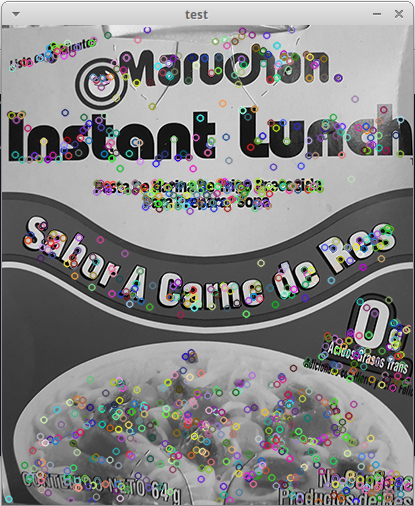
\includegraphics[width=\textwidth]{img/sopa.png}
        \caption{Sopa}
    \end{subfigure}
    ~ %add desired spacing between images, e. g. ~, \quad, \qquad, \hfill etc. 
      \begin{subfigure}[b]{0.2\textwidth}
        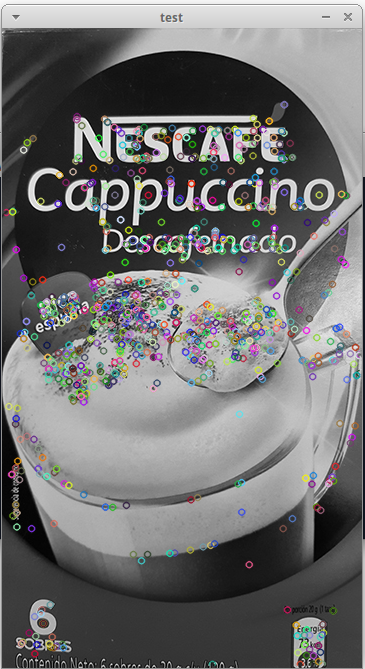
\includegraphics[width=\textwidth]{img/cafe.png}
        \caption{Café}
    \end{subfigure}

    \begin{subfigure}[b]{0.35\textwidth}
        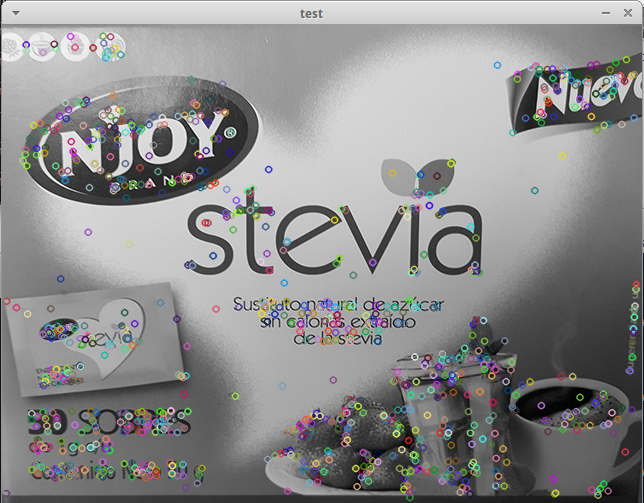
\includegraphics[width=\textwidth]{img/stevia.png}
        \caption{Stevia}
    \end{subfigure}
    ~ %add desired spacing between images, e. g. ~, \quad, \qquad, \hfill etc. 
      \begin{subfigure}[b]{0.35\textwidth}
        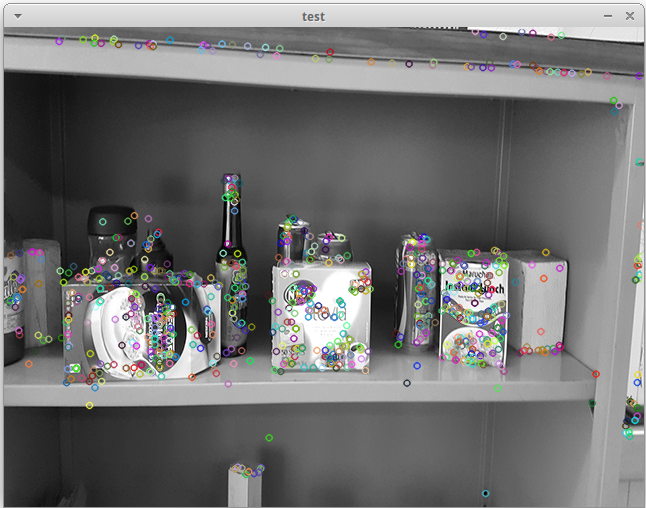
\includegraphics[width=\textwidth]{img/estante.png}
        \caption{Estante}
    \end{subfigure}
    \caption{Puntos característicos encontrados}
\end{figure}
Lo que se hizo fue medir cuánto tiempo se tardaban en generar los puntos característicos en las 3 implementaciones anteriormente mencionadas y cambiar las resoluciones de estas imágenes, porque el robot no siempre vera los objetos del mismo tamaño. Dependerá de la cámara que se esté usando o que tan lejos esté viendo los objetos. Los resultados los podemos ver a continuación en las siguientes tablas:
\begin{table}[phtb]
\centering
\begin{tabular}{|c|c|c|c|c|}
\hline
\multicolumn{5}{|c|}{Stevia} \\
\cline{1-5}
Resolución & CUDA SIFT & Open SIFT & Opencv SIFT & Puntos Característicos\\
\hline \hline
 320 x 240 px  & 31.87 ms   &   151.10 ms  &  49.42 ms   & 370\\ \cline{1-5}
 640 x 480 px  & 97.91 ms   &   484.64 ms  &  182.46 ms  & 920\\ \cline{1-5}
1280 x 960 px  & 335.05 ms  &  1751.10 ms  &  679.60 ms  & 2800\\ \cline{1-5}
2560 x 1920 px & 1251.38 ms &  5911.26 ms  &  2893.68 ms & 3000\\ \cline{1-5}
\end{tabular}
\caption{Tiempo de ejecución de la implementación en paralelo y 2 más de forma secuencial}
\label{tabla:final}
\end{table}
\begin{table}[phtb]
\centering
\begin{tabular}{|c|c|c|c|c|}
\hline
\multicolumn{3}{|c|}{Stevia} \\
\cline{1-3}
Resolución & Open SIFT/CUDA SIFT & Opencv SIFT/CUDA SIFT \\
\hline \hline
 320 x 240 px  &  4.74  &  1.55   \\ \cline{1-3}
 640 x 480 px  &  4.94  &  1.86  \\ \cline{1-3}
1280 x 960 px  &  5.22  &  2.02  \\ \cline{1-3}
2560 x 1920 px &  4.72  &  2.31 \\ \cline{1-3}
\end{tabular}
\caption{Speedup la implementación en paralelo y 2 más de forma secuencial}
\label{tabla:final}
\end{table}

\begin{table}[phtb]
\centering
\begin{tabular}{|c|c|c|c|c|}
\hline
\multicolumn{5}{|c|}{Café} \\
\cline{1-5}
Resolución & CUDA SIFT & Open SIFT & Opencv SIFT & Puntos Característicos\\
\hline \hline
 320 x 180 px  & 30.25 ms  &  117.95 ms  & 39.25 ms   & 290\\ \cline{1-5}
 640 x 360 px  & 81.91 ms  &  484.64 ms  & 182.46 ms  & 760\\ \cline{1-5}
1280 x 720 px  & 284.57 ms &  1415.27 ms & 518.27 ms  & 2800\\ \cline{1-5}
2560 x 1440 px & 993.96 ms &  4963.27 ms & 1951.21 ms & 7000\\ \cline{1-5}
\end{tabular}
\caption{Tiempo de ejecución de la implementación en paralelo y 2 más de forma secuencial}
\label{tabla:final}
\end{table}

\begin{table}[phtb]
\centering
\begin{tabular}{|c|c|c|c|c|}
\hline
\multicolumn{3}{|c|}{Café} \\
\cline{1-3}
Resolución & Open SIFT/CUDA SIFT & Opencv SIFT/CUDA SIFT \\
\hline \hline
 320 x 240 px  & 3.89   &  1.29   \\ \cline{1-3}
 640 x 480 px  & 5.91   &  2.22  \\ \cline{1-3}
1280 x 960 px  & 4.97   &  1.82  \\ \cline{1-3}
2560 x 1920 px & 4.99   &  1.96 \\ \cline{1-3}
\end{tabular}
\caption{Speedup la implementación en paralelo y 2 más de forma secuencial}
\label{tabla:final}
\end{table}

\begin{table}[phtb]
\centering
\begin{tabular}{|c|c|c|c|c|}
\hline
\multicolumn{5}{|c|}{Sopa} \\
\cline{1-5}
Resolución & CUDA SIFT & Open SIFT & Opencv SIFT & Puntos Característicos\\
\hline \hline
 206 x 240 px  & 28.10 ms  &  130.98 ms  & 37.78 ms   & 425\\ \cline{1-5}
 411 x 480 px  & 74.43 ms  &  412.04 ms  & 129.49 ms  & 1000\\ \cline{1-5}
 802 x 906 px  & 241.83 ms &  1400.59 ms & 469.07 ms  & 3000\\ \cline{1-5}
1645 x 1920 px & 850.29 ms &  4478.54 ms & 1674.67 ms & 3900\\ \cline{1-5}
\end{tabular}
\caption{Tiempo de ejecución de la implementación en paralelo y 2 más de forma secuencial}
\label{tabla:final}
\end{table}

\begin{table}[phtb]
\centering
\begin{tabular}{|c|c|c|c|c|}
\hline
\multicolumn{3}{|c|}{Sopa} \\
\cline{1-3}
Resolución & Open SIFT/CUDA SIFT & Opencv SIFT/CUDA SIFT \\
\hline \hline
 320 x 240 px  &  4.66  &  1.34   \\ \cline{1-3}
 640 x 480 px  &  5.54  &  1.73  \\ \cline{1-3}
1280 x 960 px  &  5.79  &  1.93  \\ \cline{1-3}
2560 x 1920 px &  5.26  &  1.96 \\ \cline{1-3}
\end{tabular}
\caption{Speedup la implementación en paralelo y 2 más de forma secuencial}
\label{tabla:final}
\end{table}

\begin{table}[phtb]
\centering
\begin{tabular}{|c|c|c|c|c|}
\hline
\multicolumn{5}{|c|}{Estante} \\
\cline{1-5}
Resolución & CUDA SIFT & Open SIFT & Opencv SIFT & Puntos Característicos\\
\hline \hline
 320 x 240 px  & 33.45 ms   & 130.24 ms   & 47.52 ms   & 210\\ \cline{1-5}
 640 x 480 px  & 101.20 ms  &  451.39 ms  & 177.28 ms  & 700\\ \cline{1-5}
1280 x 960 px  & 340.92 ms  &  1602.51 ms & 669.09 ms  & 2100\\ \cline{1-5}
2560 x 1920 px & 1275.37 ms &  6031.39 ms & 3037.60 ms & 3700\\ \cline{1-5}
\end{tabular}
\caption{Tiempo de ejecución de la implementación en paralelo y 2 más de forma secuencial}
\label{tabla:final}
\end{table}
\begin{table}[phtb]
\centering
\begin{tabular}{|c|c|c|c|c|}
\hline
\multicolumn{3}{|c|}{Estante} \\
\cline{1-3}
Resolución & Open SIFT/CUDA SIFT & Opencv SIFT/CUDA SIFT \\
\hline \hline
 320 x 240 px  &  3.89  &  1.42   \\ \cline{1-3}
 640 x 480 px  &  4.46  &  1.75  \\ \cline{1-3}
1280 x 960 px  &  4.70  &  1.96  \\ \cline{1-3}
2560 x 1920 px &  4.73  &  2.38 \\ \cline{1-3}
\end{tabular}
\caption{Speedup la implementación en paralelo y 2 más de forma secuencial}
\label{tabla:final}
\end{table}
\pagebreak
Un factor que pudo afectar el tiempo de ejecución de todos los programas fue la cantidad de puntos característicos que existen en la imagen, cosa que no pasó. Se puede observar cómo se repite el fenómeno que notamos con el castor y el gato. Entre más grande es la imagen obtenemos un desempeño más grande, esto paso para todos los casos en las imágenes anteriores. Es importante mencionar que el tiempo medido en las tablas incluye el cuello de botella que existe al estar pasando datos de la memoria RAM de la computadora a la memoria de la GPU.
